\documentclass[../Thesis.tex]{subfiles}
\begin{document}
	
	\section{State of the Art Review}
	\label{sec:state_of_the_art_review}
	
	Calculating the GED with traditional imperative algorithm is possible but feasible only for graphs of modest size. GED is a NP-HARD problems and for traditional solutions there is no way except to compare graphs node by node and edge by edge through combinatorial techniques to find a solution. However, as the number of nodes in the graphs increase, the complexity of these methods grows exponentially, leading to scalability issues thus infeasibility. To overcome these limitations recent works involve the use of artificial intelligence techniques such as neural networks to predict the GED between two graphs. AI-based approaches usually offer more robust and scalable solutions by learning patterns and features from graphs, significantly reducing computation times. This section reviews some of the most important papers dealing with GED calculation from 2019 to the time of writing this (2024).

	A timeline of significant works, beginning in 2019 with \textit{SimGNN} \cite{simgnn__a_neural_network_approach_to_fast_graph_similarity_computation}, the first to use neural networks for GED computation, is discussed in \autoref{sec:timeline}. Following \textit{SimGNN}, numerous models have been developed, each trying to offer something new and better performances. The timeline concludes with the most recent and promising model, \textit{GedGNN} \cite{computing_graph_edit_distance_via_neural_graph_matching}. Although these models strive to estimate GED between graphs accurately, as will be shown, this area is still in the early stages of development.
	
	
	\subsection{Timeline}
	\label{sec:timeline}
	
	2019, \textit{SimGNN: SimGNN: A Neural Network Approach to Fast Graph Similarity Computation} \cite{simgnn__a_neural_network_approach_to_fast_graph_similarity_computation}: Presents the SimGNN to solve the problem of graph similarity using neural networks. It uses a learnable embedding function, an attention mechanism to capture important nodes, and a pairwise node comparison, which is more general and efficient than the baselines.
	
	2020, \textit{Learning Graph Edit Distance by Graph Neural Networks} \cite{learning_graph_edit_distance_by_graph_neural_networks}: Presents a framework that integrates deep metric learning with the conventional approximations of graph edit distance using geometric deep learning. The approach uses a message passing neural network (MPNN) to encode graph structure and compute graph distances effectively, achieving state-of-the-art performance in graph retrieval and competitive results in graph similarity learning.
	
	2020, \textit{Combinatorial Learning of Graph Edit Distance via Dynamic Embedding} \cite{combinatorial_learning_of_graph_edit_distance_via_dynamic_embedding}: Proposes a new method to solve the GED problem through a combination of dynamic graph embedding network and an edit path search method to improve the interpretability and the efficiency of the approach. The learning-based A* algorithm decreases the size of the search tree and time while providing a minor decrease in the solution quality.
	
	2021, \textit{Graph Partitioning and Graph Neural Network-Based Hierarchical Graph Matching for Graph Similarity Computation} \cite{graph_partitioning_and_graph_neural_network_based_hierarchical_graph_matching_for_graph_similarity_computation}: Presents PSimGNN that first divides input graphs into subgraphs to learn local structural patterns and then employs a new GNN with attention to map subgraphs to embeddings and then combines coarse-grained interaction between subgraphs with fine-grained node-wise comparison to estimate similarity scores.
	
	2021, \textit{Noah: Noah: Neural Optimized A* Search Algorithm for Graph Edit Distance Computation} \cite{noah__neural_optimized_a*_search_algorithm_for_graph_edit_distance_computation}: Presents Noah that uses A* search and GPN for approximate GED calculation. Noah estimates the cost function using GPN, includes pre-training with attention-based information, and uses an elastic beam size to decrease the search space.
	
	2021, \textit{Learning Efficient Hash Codes for Fast Graph-Based Data Similarity Retrieval} \cite{learning_efficient_hash_codes_for_fast_graph_based_data_similarity_retrieval}: Proposes HGNN (Hash Graph Neural Network) that is a model for efficient graph-based data retrieval using GNNs and hash learning algorithms. HGNN learns a similarity-preserving graph representation and then generates short hash codes for efficient retrieval and classification.
	
	2021, \textit{More Interpretable Graph Similarity Computation via Maximum Common Subgraph Inference} \cite{more_interpretable_graph_similarity_computation_via_maximum_common_subgraph_inference}: Presents INFMCS, an end-to-end framework for graph similarity learning with an interpretable similarity score that is based on the correlation between the score and the Maximum Common Subgraph (MCS), and combines transformer encoder layers with graph convolution for high accuracy and interpretability.
	
	2021, \textit{H2MN: Graph Similarity Learning with Hierarchical Hypergraph Matching Networks} \cite{h2mn__graph_similarity_learning_with_hierarchical_hypergraph_matching_networks}: Presents H2MN, which computes the similarity of graph-structured data by converting graphs to hypergraphs and performing subgraph matching at the hyperedge level, and then a multi-perspective cross-graph matching layer.
	
	2022, \textit{TaGSim: Type-aware Graph Similarity Learning and Computation} \cite{TaGSim_type_aware_graph_similarity_learning_and_computation}: This work introduces TaGSim, a type-aware graph similarity learning and computation approach that overcomes the drawbacks of traditional GED methods by incorporating type-specific graph edit operations. TaGSim models the effects of various graph modifications (node and edge insertions, deletions, and relabelings) as separate operations, which generate type-aware embeddings and use them for estimating the GED. The framework outperforms other GED solutions on real-world datasets as shown in the framework.
	
	2023, \textit{Efficient Graph Edit Distance Computation Using Isomorphic Vertices} \cite{efficient_graph_edit_distance_computation_using_isomorphic_vertices}: Introduces a new strategy for the reduction of the search space of GED computation through the identification of isomorphic vertices, aiming at the elimination of unnecessary vertex mappings and thus a substantial reduction of the computation time for exact GED.
	
	2023, \textit{Exploring Attention Mechanism for Graph Similarity Learning} \cite{exploring_attention_mechanism_for_graph_similarity_learning}: Introduces a single model with attention mechanisms for node embedding, cross-graph co-attention for interaction modeling, and graph similarity matrix learning for score prediction and outperforms the state of the art on benchmark datasets.
	
	2023, \textit{Graph Edit Distance Learning via Different Attention} \cite{graph_edit_distance_learning_via_different_attention}: Proposes DiffAtt, a new graph-level fusion module for GNNs to compute GED efficiently with the help of structural differences between graphs using attention, integrated into the GSC model REDRAFT, which outperforms the state of the art on benchmark datasets.
	
	2023, \textit{Graph-Graph Context Dependency Attention for Graph Edit Distance} \cite{graph_graph_context_dependency_attention_for_graph_edit_distance}: Presents GED-CDA, a deep network architecture for GED computation which uses a graph-graph context dependency attention module that combines cross-attention and self-attention layers to model inter-graph and intra-graph dependencies.
	
	2023, \textit{GREED: A Neural Framework for Learning Graph Distance Functions}: Introduces GREED, a siamese GNN for learning GED and SED in a property preserving manner which outperforms other methods in terms of accuracy and time complexity.
	
	2023, \textit{MATA*: Learnable Node Matching with A* Algorithm for Approximate Graph Edit Distance} \cite{mata_combining_learnable_node_matching_with_a*_algorithm_for_approximate_graph_edit_distance}: Presents MATA*, a novel approach for the approximate GED computation that combines GNNs and the A* algorithm, with the focus on learning the node matching.
	
	2023, \textit{Multilevel Graph Matching Networks for Deep Graph Similarity Learning} \cite{multilevel_graph_matching_networks_for_deep_graph_similarity_learning}: Introduces MGMN, a multilevel graph matching network that can capture the cross-level interactions, which includes NGMN and a siamese GNN for global-level interactions, and performs well when graph sizes are large.
	
	2023, \textit{Wasserstein Graph Distance Based on L1-Approximated Tree Edit Distance Between Weisfeiler-Lehman Subtrees} \cite{wasserstein_graph_distance_based_on_l1_approximated_tree_edit_distance_between_weisfeiler_lehman_subtrees}: Introduces the WWLS distance which integrates WL subtrees with L1-TED which is more sensitive to fine changes in the structure of graphs and outperforms other methods in metric validation and graph classification.
	
	2023, \textit{Computing Graph Edit Distance via Neural Graph Matching} \cite{computing_graph_edit_distance_via_neural_graph_matching}: Presents GEDGNN, a deep learning model for GED computation that works on the idea of graph transformation instead of directly predicting GED value. GEDGNN provides GED values and a matching matrix and a post-processing procedure for obtaining high quality node mappings.
	
	\subsection{SimGNN}
	\label{sec:simgnn}
	
	The first innovative model that used neural networks is SimGNN \cite{simgnn__a_neural_network_approach_to_fast_graph_similarity_computation}, introduced in 2019. SimGNN serves as a foundational model in the field of graph similarity computation, in fact future models will often inherit its core concepts (such as the siamese layout architecture), making it the starting point of reference for anyone dealing with GED computation. 
	
	The architecture of SimGNN [\autoref{fig:simgnn_architecture}] is composed by several stages:
	
	\begin{itemize}
		\item \textbf{Node Embedding Stage}: This stage makes use of a graph convolutional network to capture local structural information that transforms each node in the graph into a vector that encodes its features and structural properties.
		\item \textbf{Graph-Level Embedding Stage}: This stage produces a single embedding representing the whole graphs starting from the previously produced nodes embeddings by also using attention mechanisms to focus on important nodes.
		\item \textbf{Graph-Graph Interaction Stage}: This stage puts in communication the two graphs embedding previously produced and produces a matrix of similarity interaction scores.
		\item \textbf{Final Similarity Score Computation Stage}: This stage process the previously produced similarity matrix to compute the final similarity score.
	\end{itemize}
	
	In addition to the graph-level embedding interaction strategy, SimGNN has a its disposal a pairwise node comparison strategy:
	
	\begin{itemize}
		\item \textbf{Pairwise Node Comparison}: This strategy involves computing pairwise interaction scores between the node embeddings of the two graphs. The resulting similarity matrix is used to extract histogram features, which are then combined with the graph-level interaction scores to provide a comprehensive view of graph similarity.
	\end{itemize}
	
	The combination of these two strategies should allow the model to capture both global and local informations which should result in a robust approach to graph similarity computation.
	
	\begin{figure}[H]
		\centering
		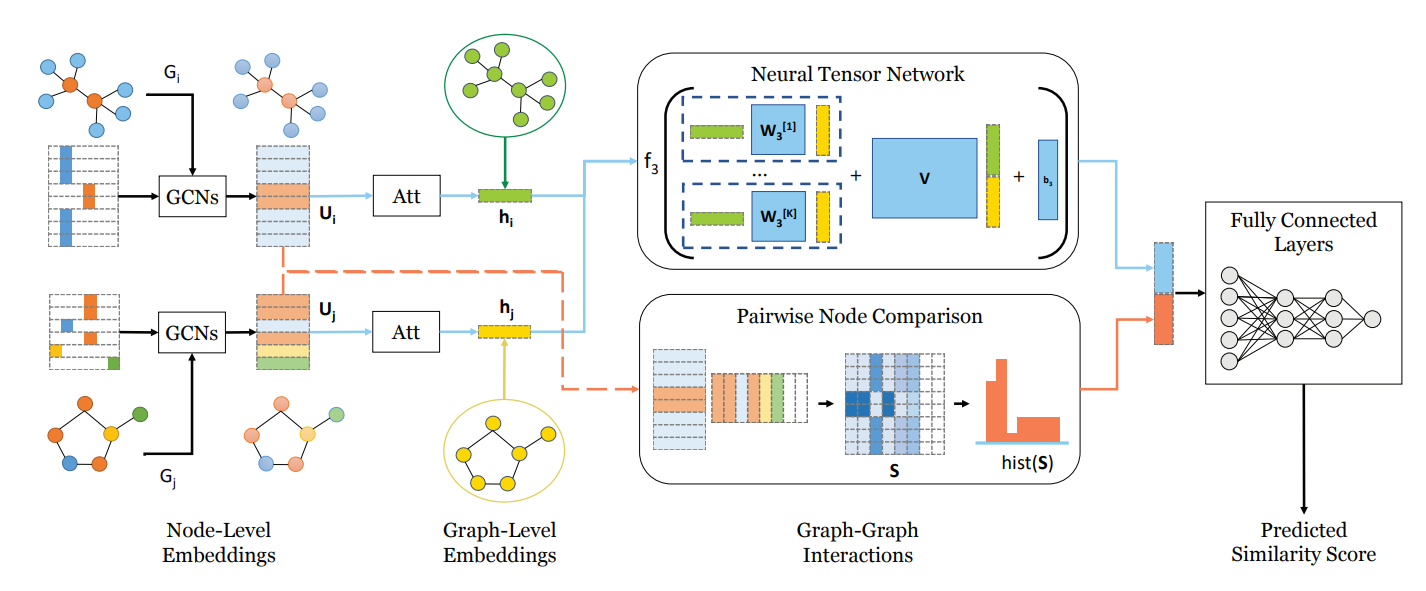
\includegraphics[width=\textwidth]{Images/simgnn_architecture.png}
		\caption{SimGNN architecture overview.}
		\label{fig:simgnn_architecture}
	\end{figure}

	
	\subsection{GPN}
	\label{sec:gpn}
	
	In 2022, an innovative hybrid approach for computing GED was released.
	The Graph Path Networks (GPN) model, proposed within the \textit{NOAH Framework} \cite{noah__neural_optimized_a*_search_algorithm_for_graph_edit_distance_computation}, introduces the GED computation by exploiting the A* search algorithm optimized through neural networks. This method tries to address several previously found limitations trying to improve both the search direction and search space optimization.
	
	The architecture of GPN [\autoref{fig:gpn_architecture}] is composed by several modules:
	
	\begin{itemize}
		\item \textbf{Pre-training Module}: This module computes pre-training information about the graphs that will be exploited by the next modules.
		\item \textbf{Graph Embedding Module}: This module utilizes layers of Graph Isomorphism Network (GIN) to transform each node into a vector. Then these embeddings are combined into a single graph level embedding by using different attention mechanisms.
		\item \textbf{Learning Module}: This module focuses on optimizing the A* search algorithm by learning an estimated cost function and an elastic beam size. The tradition algorithm is then used for the final prediction.
	\end{itemize}
	
	The main advantage of GPN over SimGNN is that it is capable of finding an edit path between graphs (roughly accurate) between graphs in a short amount of time.
	
	\begin{figure}[H]
		\centering
		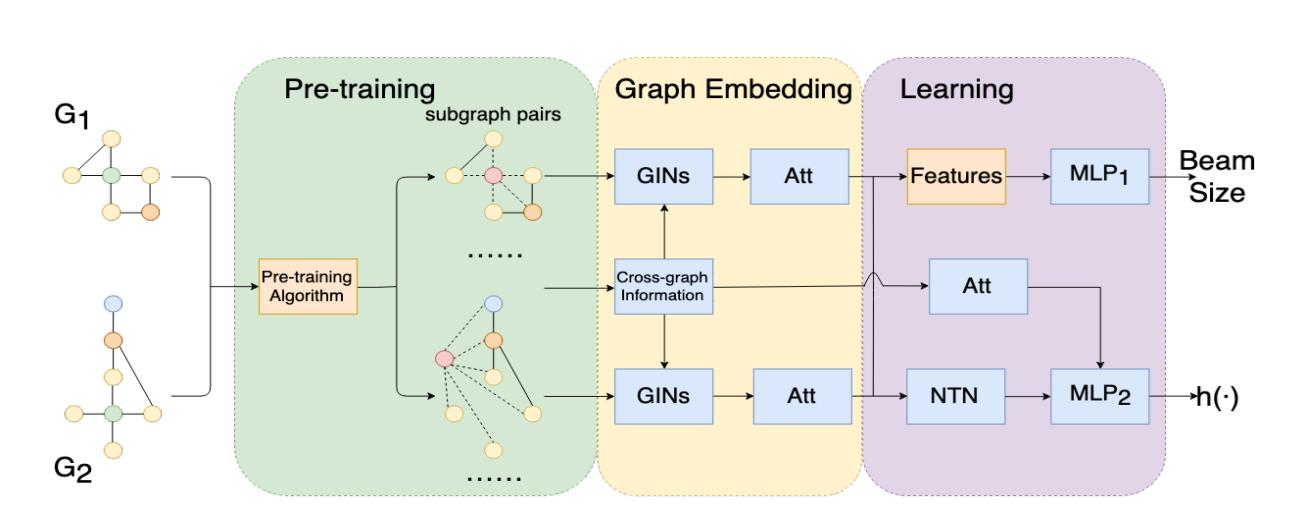
\includegraphics[width=\textwidth]{Images/gpn_architecture.png}
		\caption{GPN architecture overview.}
		\label{fig:gpn_architecture}
	\end{figure}
	
	
	\subsection{TaGSim}
	\label{sec:tagsim}
	
	In 2022, another innovative approach was released with TaGSim (Type-aware Graph Similarity) \cite{TaGSim_type_aware_graph_similarity_learning_and_computation}. The idea behind GED as a single value has been revaluated and it is now thought as the summation of three different values: $ged\_nc$ the number of node relabelling, $ged\_in$ the number of node insertions/deletions, $ged\_ie$ the number of edges insertions/deletions. 
	
	The architecture of TaGSim [\autoref{fig:tagsim_architecture}] is composed by several components:
	
	\begin{itemize}
		\item \textbf{Type-Aware Graph Embeddings}: This component takes into account the different impacts that different atomic operations could have when predicting the GED producing a type-aware graph level embedding. Namely the operations taken into accounts are: node insertion/deletion (NR), node relabeling (NID), edge insertion/deletion (ER), and edge relabeling (EID). Each type of operation is handled separately to capture its localized effects on the graph.
		\item \textbf{Type-Aware Neural Networks}: This component takes advantage of specific neural networks that are specifically designed to process and learn from the type-aware embeddings. This allows TaGSim to achieve high accuracy in GED estimation by incorporating the distinct impacts of different edit types and outputs them all.
	\end{itemize}
	
	The main advantage of TaGSim over predecessors is that by decoupling the GED into different dimensions, there is the potential for more granular control and learnability.
	
	\begin{figure}[H]
		\centering
		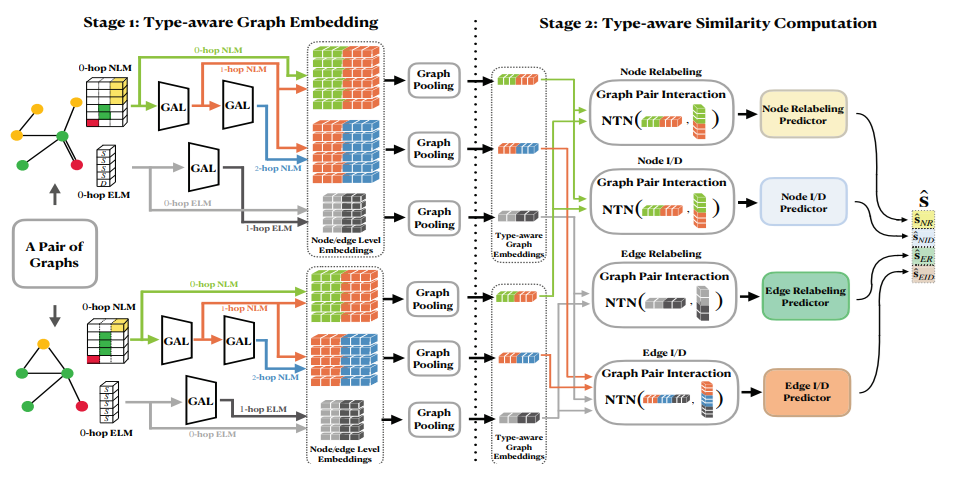
\includegraphics[width=\textwidth]{Images/tagsim_architecture.png}
		\caption{TaGSim architecture overview.}
		\label{fig:tagsim_architecture}
	\end{figure}

	\subsection{GedGNN}
	\label{sec:gedgnn}
	
	In 2023, the model that is considered the state of the art at the time of writing this (2024) is released with GedGNN (Graph Edit Distance via Neural Graph Matching) \cite{computing_graph_edit_distance_via_neural_graph_matching}. The idea behind this model is to try to put together all the best ideas from past's models including the basic siamese layout of SimGNN, the use of more advanced convolutional layers of GPN and the split of the GED metric from TaGSim while still allowing for the retrieval of an edit paths by taking inspiration from NOAH framework.
	
	The architecture of GedGNN [\autoref{fig:gedgnn_architecture}] is composed by several components:
	
	\begin{itemize}
		\item \textbf{Graph Neural Network (GNN) Encoder}: This component produces the encodings for nodes and edges while preserving their relational information. This is done through the employment of an advanced GNN encoder.
		\item \textbf{Node and Edge Matching Module}: This component performs the node and edge matching between the pair of graphs producing a matching matrix and a cost matrix.
		\item \textbf{k-Best Matching Post-Processing Algorithm}: After predicting the GED value a k-best post-processing algorithm is used trying to retrieve a good edit path.
	\end{itemize}
	
	GedGNN's results state to not only outperforms previous methods but also provides a flexible framework that can adapt to various types of graph structures and similarity measures.
	
	\begin{figure}[H]
		\centering
		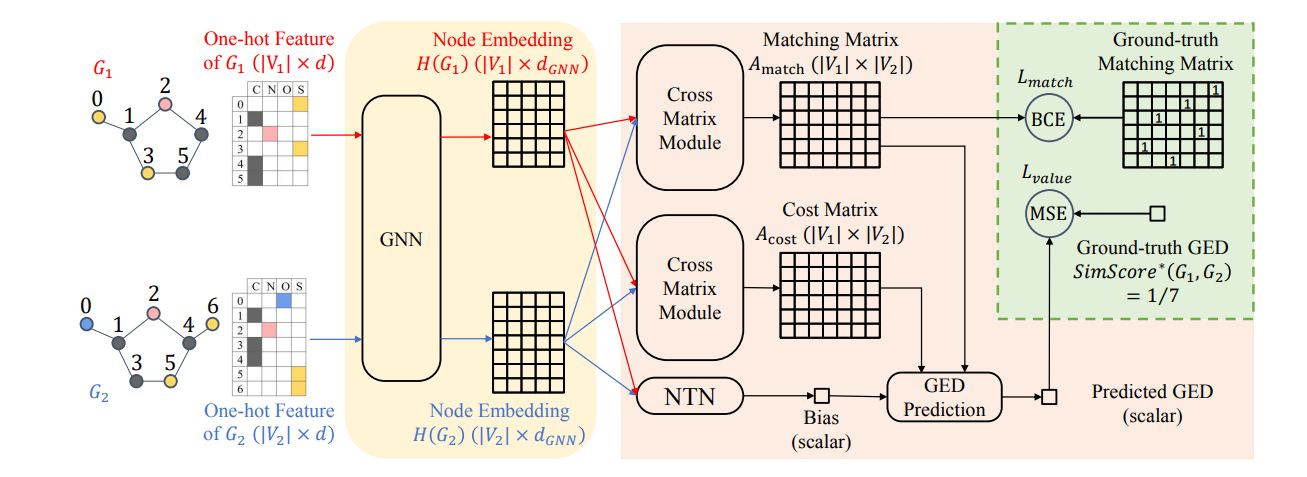
\includegraphics[width=\textwidth]{Images/gedgnn_architecture.png}
		\caption{GedGNN architecture overview.}
		\label{fig:gedgnn_architecture}
	\end{figure}
	
	\subsection{Encountered Gaps}
	
	In this research, some problems and concerns have been identified from the \href{https://github.com/ChengzhiPiao/GEDGNN}{codebase} of GedGNN. Most of these issues can be attributed to the fact that codes are copied from one project to another and reused by researchers without proper testing.
	
	The first problem is related to the code quality of the codebase. It is often poor and there is also no strong adherence to best practices. There are numerous method implementations that look very much like they do the same thing, too many classes, numerous questions, and no way of handling the errors. In some parts, the code appears to have been almost hard coded, thus, offers little room for modification. Also, the code can be hardly understood, and the comments that are given with the code are quite uninformative.
	
	Closely related to code quality and testing scenarios is the problem of scalability on GPUs. When trying to run for the first time the code as is on a GPU some errors also raised up, but apart from this, the models do not scale well on GPU hardware and this is an issue. Training on small datasets is possible on CPUs but when it comes to using large datasets for testing and training new models, issues arise with long training time per epoch.
	
	Another concern is that the codebase only permits the use of graphs with 10 nodes or less in training, testing, and validation cases. This could be attributed to the fact that there are complex imperative algorithms that are used in the software such as the k-best post-processing algorithm for reconstructing edit paths. In addition, for any model, the code fails when tested on the IMDB dataset. Additionally, despite the presence of artificial dataset generation code, it is not utilized, leading to confusion and unreachable code paths.

	The training data, however, has issues that have been there from the time SimGNN was created. The same datasets are used over and over again, however, the most important problem is that approximate GEDs are used as labels instead of the exact one. These datasets are relatively small; graphs contain less than ten nodes, and with today’s hardware, we would not spend much time calculating exact GED. Also, in all codebases analyzed so far, the training is done in a way that for each pair of graphs in the training set there is a corresponding GED.
	
	However, the biggest problem has to do with the fact that there is no fair testing between models. It is still not well understood why so, but with the current state of the codebase, one cannot even attempt to test a model trained on one dataset with another dataset. This restriction may be to hide the fact that there is no generalization capability.
	
	In summary, the analysed codebase which presents GedGNN, TaGSim, SimGNN and GPN presents several significant challenges to overcome. These include problems with the reproducibility of the results, fair evaluations, scalability issues, poor code quality, unclear parameters and more. Clearly, resolving many of this issues would lead to a significant advancement in this field.
	
\end{document}
